\documentclass[titlepage,a4paper]{article}
\usepackage[mathletters]{ucs}
\usepackage[utf8x]{inputenc}
\usepackage[margin=3cm]{geometry}
\usepackage{fancyhdr,graphicx,hyperref,tipa,bm}

\setlength{\headheight}{15.2pt}
\pagestyle{fancy}
\newcommand{\HRule}{\rule{\linewidth}{0.5mm}}

\begin{document}
% 1. Title page
\begin{titlepage}
\begin{center}

\textsc{\LARGE COMPGS04/M024: Tools and Environments}\\[2cm]

\HRule \\[0.4cm]
{ \huge \bfseries Coursework 2 (Group Coursework) \\[0.4cm] }

\HRule \\[1.5cm]

\large\emph{Authors:}\\
Jihyun \textsc{Han}\\
Elliott \textsc{Omosheye}\\
Sachin \textsc{Pande}\\
Luke \textsc{Richardson}\\
Yasaman \textsc{Sepanj}

\vfill
{\large \today}
\end{center}
\end{titlepage}

% 2. Introduction to problem
% Introduction

\section{Introduction}
\subsection{Background}
In software engineering, cloned code is one of the fundamental issues of productivity. The programming community is generally recognising the duplicates as a bad practice [Refactoring: Improving the Design of Existing Code by Martin Fowler], although some argue otherwise. We tend to avoid it because we are taught that repeated code is inelegant and can cause difficulties whilst trying to maintain applications, or sometimes it may involve legal risks. However, due to time pressure, or limitation of programming languages, reusing code fragments by duplicating with or without variations is a common activity evident within software development.

Unlike plagiarism detection in literature, duplicated code does not solely depend on text matching, but consideration has to be made for the syntax, semantics and patterns of the codes. For instance, two source files that functions the same may have completely different identifier names for variables – this must also be detected as a clone. Different approaches to achieve the detection exists, and will be discussed later.
\subsection{Project}
In a 5 membered team, we are given the task of building a tool that analyses and reports similarity of two Java source files. This report introduces 5 different similarity detection mechanisms including Clone Detection and Plagiarism Detection, and we shall decide a suitable algorithm to implement for the tool. The tool will be tested with a given sample code and its variations to check our program’s performance whilst analysing the similarities between the pair of codes.

\break

% 3. Summary of paper 1 (Jihyun)
\section{Normalized Compression Distance}
\href{http://arxiv.org/ftp/arxiv/papers/0809/0809.2553.pdf}{Vit\'{a}nyi, Paul MB and Balbach, Frank J and Cilibrasi, Rudi L and Li, Ming. Information theory and statistical learning: Normalized Information Distance. Springer. 2009.}
\subsection{Background}
Normalized compression distance is a method of computing the similarity between two documents of any kind whether this be two text files or two music files. It measures the difficulty of being able to turn one document to the other. This method of determining similarities between two files is based upon the Normalized Information Distance (NID) between them.

\subsection{Normalized Information Distance}
The information distance between two strings $\boldsymbol{x}$ and $\boldsymbol{y}$ is defined to be the length of the shortest program, $\boldsymbol{p}$, for a universal computer to transform $\boldsymbol{x}$ into $\boldsymbol{y}$ and vice versa. The length of this program can be defined with the use of Kolmogorov complexity as follows:\\
\begin{equation}
\boldsymbol{|p| = \mathbf{max}\{K(x|y),K(y|x)\}}
\end{equation}
This distance is absolute and therefore needs to be normalized in order to provide the similarity in relative to both the files. Such an normalization provides the NID. \\
\begin{equation}
\boldsymbol{e(x,y) = \frac{\mathbf{max}\{K(x|y),K(y|x)\}}{\mathbf{max}\{K(x),K(y)\}}}
\end{equation}

\subsection{Normalized Compression Distance}
The NID is however impractical as it uncomputable. Therefore requiring a computable algorithm is requires, such a algorithm is Normalized Compression Distance (NCD). Transforming the equation through substitution of the uncomputable function $\boldsymbol{K}$ with a real-world compression function $\boldsymbol{Z}$ provides the NCD, defines by
\begin{equation}
\boldsymbol{e_{Z}(x,y) = \frac{Z(xy)-\mathbf{min}\{Z(x),Z(y)\}}{\mathbf{max}\{Z(x),Z(y)\}}}
\end{equation}
where $\boldsymbol{Z(x)}$ is the length of the compression of string $\boldsymbol{x}$ using the compression function $\boldsymbol{Z}$.

\subsection{Application}
For the case of this project we are interested in similarities between Java source files, for which a variant of the NID can be used to measure the similarity. This variant named sum distance is defined by
\begin{equation}
    \boldsymbol{e_{\mathbf{sum}}(x,y) = \frac{K(x|y)+K(y|x)}{K(x,y)}}
\end{equation}
The two files are tokenized then compressed with a customized compressor to approximate the sum distance. 

\subsection{Conclusion}
NCD is able to provide a good score for the similarity between two files. Whilst the NCD algorithm and the variant sum distance are relatively easy to implement, the latter requires the need for the implementation of a custom compressor which is out of scope for this project. Furthermore these algorithms are unable to provide details about the nature of the similarities between the two Java source files. \\
\break

% 4. Summary of paper 2 (Elliott)
\section{Plagiarism Detection}

\subsection{Introduction}
Plagiarism detection in code is the method and process used for locating instances of cloned code within a set of documents. The tool we have chosen to demonstrate and explore plagiarism detection is JPlag. 

\subsection{JPlag}
JPlag is a system that finds similarities, software plagiarisms, among multiple source code files. It is robust against many attempts to disguise the copied code because it is aware of programming language syntax and program structure. Thus, it is very hard to deceive: 90\% of plagiarisms are detected and the rest raise suspicion. [1] Moreover, JPlag is able to process a hundred programs with several hundred lines of code in seconds, making it a very robust and scalable tool. 
It has been successfully used for detecting plagiarism among students’ Java programs but support for other languages such as C and C++ are also available.\\\\
JPlag’s comparison algorithm is based on the “Greedy String Tiling” [2], which takes in a set of program source code as input and outputs a similarity score between pairs of programs and their corresponding similarity regions. To do so, it must initially convert the program source code in to token strings, this is the only language dependent process involve din JPlag’s plagiarism detection. Tokens should be chosen in a manner, which captures the essence of the program’s structure rather than the surface aspects, as a program’s structure is harder for plagiarists to modify. JPlag does this phase whilst ignoring whitespaces, comments and names of identifiers. Figure \ref{fig:sample} shows an example Java code and its corresponding tokens generated by JPlag. A list of possible JPlag tokens can be found in this technical report [3].\\\\
\begin{figure} [ht]
\centering
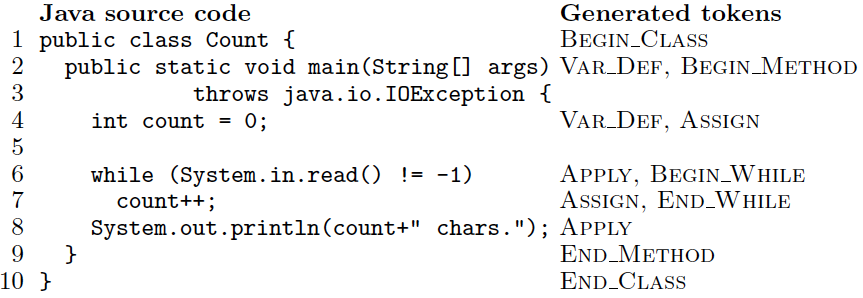
\includegraphics[width=0.7\textwidth]{Figures/samplecode}
\caption{A sample Java Source code with the generated token strings}
\label{fig:sample}
\end{figure}
Once the token strings have been generated, JPlag beings the comparison phase by comparing the two generated token strings. When comparing two strings A and B, JPlag’s objective is to discover a maximal set of contiguous substrings. Each substring must occur in both A and B and must be as long as possible. These substrings (matches) must be unique in that each substring should not cover tokens already covered by other substrings. To avoid false matches, a minimum match length M is enforced. 

\subsection{Greedy Tiling Algorithm}
The Greedy String Tiling algorithm itself has two steps shown in Figure \ref{fig:greedy}. Firstly, all substrings common to both token strings are found with lengths equal to or greater than the minimum M. Secondly, all the tokens found in the substrings are marked so that they are no longer picked up by subsequent iterations of the first step. By marking its tokens, a match becomes a “tile”. Thus, the similarity score between is calculated based on the fraction of tokens that were found as matches:

\begin{equation}
    sim(A,B) = \frac{2 * coverage(tiles)}{|A|+|B|}
\end{equation}
\begin{figure} [ht]
\centering
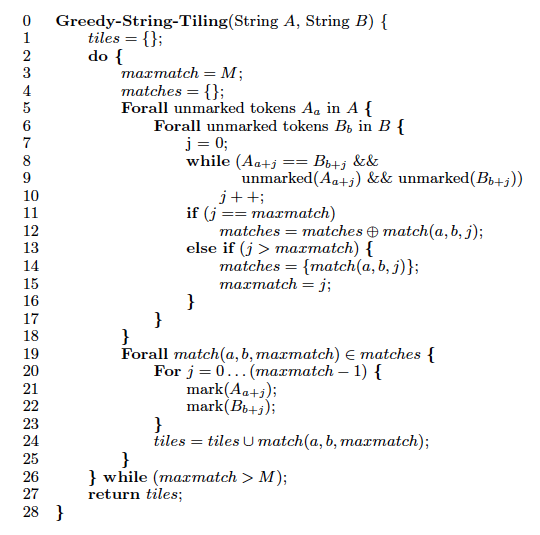
\includegraphics[width=0.7\textwidth]{Figures/stringtiling}
\caption{Greedy String Tiling algorithm}
\label{fig:greedy}
\end{figure}

\break

% 5. Summary of paper 3 (Sachin)
\section{Paper 3}

\subsection{Sub-section}
\break

% 6. Summary of paper 4 (Luke)
\section{Paper 4}

\subsection{Sub-section}
\break

% 7. Summary of paper 5 (Yasaman)
\section{Measuring similarity using Clone Detection approach}
One of the approaches to detecting similarity in code is the Clone Detection. It is able to find the similarities between the code files and also provide the position of duplicates.

\subsection{Code Detection}
Typically, clone detection is done by comparing the two streams of data and spotting out any identical segments that exists in both of the streams. The comparisons can be based on text, tokens, syntax or structures.
The clone detection steps are as follows [1]:
\begin{itemize}
\item Raw code is fed into the pre-processing stage where it removes uninteresting codes such as embedded code such as SQL queries in a Java file. It determines the comparison unit such as tokens, hash or characters, etc.
\item The processed code is then transformed to the form suitable as input to the actual comparison algorithm. It can tokenize or parse depending on the comparison unit and it removes whitespaces and comments to normalise the code.
\item The transformed code is then fed into a comparison algorithm. It aims to find the longest contiguous sequence of similar units. It outputs a list of matches that were found in the transformed code.
\item It then maps the detected clones back to the source code by their line numbers.
\item Then it can be extracted from the source to be visualised for manual inspection, such as the scatter dot plot.
\item Sometimes, in order to reduce the amount of data, it can return only clone pairs as the result. 
\end{itemize}
\begin{figure} [ht]
\centering
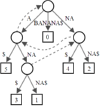
\includegraphics{Figures/clonedetection}
\caption{Clone detection}
\label{fig:clone}
\end{figure}
One of the applications that utilises clone detection is the CCFinder. It aims to be used in an industrial scale and to be applicable to million-line size system. The tool takes token sequences as comparison unit through a lexical analyser and applies rule-based transformation to the sequence, which enables the tool to be able to detect cloned code portions that have different syntax but may have similar meaning. CCFinder utilises suffix tree matching algorithm to detect clones. Suffix tree matching provides the position of the detected segments as a tree with sharing nodes that represents duplicates. CCFinder searches the leading nodes on the tree for clone detection.

\subsection{Rabin-Karp algorithm used for Clone Detection}
The native string search used for Clone Detection may be too slow as it iterates through every message space available. A variant of the algorithm is the Rabin-Karp algorithm. The algorithm is a string search algorithm created by Michael O. Rabin and Richard M. Karp, and is one of the clone detection algorithm. It calculates a hash value for a pattern and for each character substring of the given text. Instead of comparing every combinations of characters or tokens, it compares the numerical value (hash) to detect clones. The hash function returns a shortened codes compared to the raw codes, hence the speed of matching becomes faster than a brute-force string matching.[3]
\break

% 8. Tool requirements
\section{Tool requirements}

\subsection{Overview}
The following list of requirements are formed from the defined set of tool requirements in the coursework brief and based on our algorithm choice, JPLAG plagiarism detection.
\subsection{Requirements}
\begin{enumerate}
\item The tool will compute a similarity measurement for two input Java source code files using an implementation of the JPLAG plagiarism detection algorithm.

\item The tool must work via command line and should not have a graphical interface.

\item Input taken should be the names of two files as command lines arguments.

\item The output should be a similarity measure to STDOUT as a percentage.

\item Input Java source files will be parsed using a Java parser library, ANTLR.

\item The tool will be written in Java (version 6) to meet the requirements for the parser library.

\item The tool will not invoke the JPLAG binary or any other similarity testing tool.

\item The output of similarity measurement by plagiarism detection algorithm will complete in reasonable time for expected inputs. Expected inputs are generally Java source code files and specifically under testing TOH.java, variants of TOH.java and arbitrary dissimilar test inputs.

\item The tool will have an automated testing mechanism to carry out pairwise comparison of the said files.

\item The tool should work with all platforms the JVM works on that support ANTLR. The tool will be tested and run on Linux and Windows platforms.

\end{enumerate}
\break


% 9. UML Diagrams of tool architecture
\section{UML Diagrams of architecture}

\subsection{Sub-section}
\break

% 10. Implementation
\section{Implementation}
The development of the plagiarism detector involved implementing Michael Wise’s “Greedy String Tiling” algorithm, as introduced before. In order for the algorithm work flawlessly, we have prepared our own data holder classes: a “Token” class responsible for objectifying each token every loop, and a “Match” class that tracks where the duplicates were detected. The implementation of the pseudo-code of Greedy String Tiling was done in Java. Our tool’s workflow is as follows. 

\subsection{Tokenizing}
The Greedy String Tiling compares tokens instead of each characters. It is required that the tool is able to understand the source code (written in Java) and recognise the grammar. We used ANTLR and a Java grammar (from Github, under BSD licence) for ANTLR to convert the source files into token strings. Initially, the given Java grammar dealt with all Java statements in one expression. However, in order to be able to classify different semantics behind the tokens, we needed to add separate method for if statements, for loops, etc. A Listener object was created for the parser to be able to tokenize according to the aforementioned rules. The tokenized string is then passed to the main method to be manipulated for plagiarism detection.

\subsection{Algorithm}
The Java implementation of the Greedy String Tiling algorithm is as follows:
Given the list of Token objects of two source code files, set A and set B, we iterate through A and B with two nested loops. The algorithm compares the tokens to see if they are identical, and to see if the two tokens are not ‘marked’ (initially set to false). If the condition succeeds, another innermost nested loop repeats this process until the condition does not hold. While it does, it counts the how far the duplicate has extended, and creates a Match object with Index of the duplicated tokens from both sets, and the length of the duplicate - thus it eventually collects the set of all longest common substring.
The algorithm has a mechanism where it keeps only the largest duplicates. The program checks whether, in each loop, the match is at least as long as the longest ones found before, whose length is stored in maxMatch variable. If the length is equal to maxMatch, another maximal match is found and added to the global set called matches. If the length is larger than maxMatch, the global set matches is cleared and newly adds the current duplicate. The maxMatch is now the length of the current duplicate.
The global set ‘matches’ is then emptied to the result set called ‘tiles’. The matches set is cleared and the above process repeats until maxMatch is lower than a fixed threshold, which we set to be 3. As more duplicates are found, the algorithm will eventually halt when it cannot find any more duplicates that are long than length 3.

\subsection{Analysis}
The similarity percentage is calculated as follows:\\
 Coverage = sum of all lengths of duplicated codes\\
		Similarity percentage = 2 * Coverage/length of file A + length of file B\\

Higher percentages indicate a higher chance of plagiarism. It should be noted that given two identical code, if one was to add more content to one of them, the similarity percentage decreases, due to the nature of the calculation.

\break

% 11. Testing
\section{Testing}

\subsection{Sub-section}
\break

% 12. Results of pairwise comparison
\section{Results of pairwise comparison}
The pairwise comparison results are shown within the pairwisetest.txt file, listing the files tested against each other in addition to the similarity score. 

\subsection{Comparison file original file}
Whilst comparing the original file to the Type 1-4 clones, variant of TOH and dissimilar code the results seem to indicate that the application works well. However there are some outliers where one of the dissimilar files, specifically test 17, the application classes that as a highly similar file. In addition to this anomaly we found that one of the Type 3 clone, test 7, outputs a lower similarity value than expected. This seems to suggest moving and combining methods causes the application to determine that the files are largely different.
\begin{table}[h]
\begin{tabular}{|l|l|l|l|l|l|l|l|l|l|l|}
\hline
& \multicolumn{2}{|c|}{TOH} & \multicolumn{2}{|c|}{Dissimilar} & \multicolumn{2}{|c|}{Type 1} & \multicolumn{4}{|c|}{Type 2}  \\
\hline
  & 6    & 15  & 16   & 17 & 3   & 5 & 1   & 2 & 4 & 14  \\
  \hline
0 & 51\% & 48\% & 68\% & 48\% & 96\% & 100\% & 98\% & 100\% & 96\% & 99\% \\
\hline
\end{tabular}
\end{table}
\begin{table}[h]
\begin{tabular}{|l|l|l|l|l|l|l|l|}
\hline
& \multicolumn{5}{|c|}{Type 3} & \multicolumn{2}{|c|}{Type 4} \\
\hline
  & 7   & 8 & 9 & 10 & 11 & 12 & 13 \\
  \hline
0 & 49\% & 99\% & 84\% & 82\% & 82\% & 88\% & 88\% \\
\hline
\end{tabular}
\end{table}

\subsection{Comparison with dissimilar files}
The comparison of the dissimilar files, test 16, 17 with the other test files outputs some interesting results. Firstly the comparison with the test file 17 with most of the other files except a couple output a very high similarity score, which suggests the token set may be too small and therefore with a more diverse token set this problem could be rectified. The comparison with the other test file, 16 shows that the application determines dissimilar files well.
\begin{table}[h]
\begin{tabular}{|l|l|l|l|l|l|l|l|l|l|l|l|l|l|l|l|l|l|l|}
\hline
& \multicolumn{2}{|c|}{TOH} & \multicolumn{2}{|c|}{Type 1} & \multicolumn{4}{|c|}{Type 2} & \multicolumn{5}{|c|}{Type 3} & \multicolumn{2}{|c|}{Type 4} \\
\hline
  & 6    & 15  & 3   & 5 & 1   & 2 & 4 & 14 & 7   & 8 & 9 & 10 & 11 & 12 & 13  \\
  \hline
16 & 50\% & 37\% & 59\% & 61\% & 57\% & 61\% & 58\% & 63\% & 25\% & 60\% & 52\% & 54\% & 54\% & 55\% & 55\%\\
\hline
17 & 34\% & 51\% & 95\% & 95\% & 93\% & 95\% & 86\% & 91\% & 54\% & 94\% & 94\% & 94\% & 94\% & 92\% & 92\%  \\
\hline
\end{tabular}
\end{table}

\break
\subsection{Comparison with TOH variants}
The results of the pairwise comparison between the Tower of Hanoi and the clones mostly with the exception of one test file suggests that the files are most dissimilar. The anomaly being more dissimilar than the rest. This meets with the expectation since the implementation of solving tower of hanoi is considerably different to the original. One of the implementations is recursive as opposed to iterative in the original file and the other using stacks.

\begin{table}[h]
\begin{tabular}{|l|l|l|l|l|l|l|l|l|l|l|l|l|l|l|l|l|l|}
\hline
& \multicolumn{2}{|c|}{Type 1} & \multicolumn{4}{|c|}{Type 2} & \multicolumn{5}{|c|}{Type 3} & \multicolumn{2}{|c|}{Type 4} \\
\hline
  & 3   & 5 & 1   & 2 & 4 & 14 & 7   & 8 & 9 & 10 & 11 & 12 & 13 \\
  \hline
16 & 56\% & 50\% & 51\% & 50\% & 56\% & 52\% & 22\% & 56\% & 55\% & 58\% & 58\% & 59\% & 59\%  \\
\hline
16 & 34\% & 34\% & 35\% & 34\% & 33\% & 36\% & 15\% & 28\% & 35\% & 34\% & 34\% & 35\% & 35\%  \\
\hline
\end{tabular}
\end{table}



% 13. Evaluation of results and tool performance
\section{Evaluation of results and project review}

\subsection{Sub-section}
\break

% 14. Group responsibilities
\section{Responsibilites}

\subsection{}
\break

% (15. References)
\subsection{References}
$[1]$ Comparison and evaluation of code clone detection techniques and tools: A qualitative approach. Chanchal K. Roy, James R. Cordy, Rainer Koschke.\\
$[2]$ CCFinder: A Multi-Linguistic Token-based Code Clone Detection System for Large Scale Source Code. Toshihiro Kamiya, Shinji Kusumoto, Member, IEEE, and Katsuro Inoue, Member, IEEEE.\\
$[3]$ \href{http://www.stoimen.com/blog/2012/04/02/computer-algorithms-rabin-karp-string-searching/}{Computer algorithms: Rabin-Karp String Searching from Stoimen?s Web log.}\\
$[4]$ Prechelt, Lutz, Guido Malpohl, and Michael Philippsen. "Finding plagiarisms among a set of programs with JPlag." J. UCS 8.11 (2002): 1016.\\
$[5]$ \href{ftp://ftp.cs.su.oz.au/michaelw/doc/RKR GST.ps}{Michael J. Wise. String similarity via greedy string tiling and running Karp-Rabin matching, Dept. of CS, University of Sydney, December 1993.}\\
$[6]$ Prechelt, Lutz, Guido Malpohl, and Michael Philippsen. “JPlag: Finding plagiarisms among a set of programs.” Technical Report 2000-1, March 2000\\


\end{document}